

\documentclass[conference]{IEEEtran}
% Add the compsoc option for Computer Society conferences.
%
% If IEEEtran.cls has not been installed into the LaTeX system files,
% manually specify the path to it like:
% \documentclass[conference]{../sty/IEEEtran}


% Some very useful LaTeX packages include:
% (uncomment the ones you want to load)


% *** MISC UTILITY PACKAGES ***
%
%\usepackage{ifpdf}
% Heiko Oberdiek's ifpdf.sty is very useful if you need conditional
% compilation based on whether the output is pdf or dvi.
% usage:
% \ifpdf
%   % pdf code
% \else
%   % dvi code
% \fi
% The latest version of ifpdf.sty can be obtained from:
% http://www.ctan.org/tex-archive/macros/latex/contrib/oberdiek/
% Also, note that IEEEtran.cls V1.7 and later provides a builtin
% \ifCLASSINFOpdf conditional that works the same way.
% When switching from latex to pdflatex and vice-versa, the compiler may
% have to be run twice to clear warning/error messages.


% *** CITATION PACKAGES ***
%
%\usepackage{cite}
% cite.sty was written by Donald Arseneau
% V1.6 and later of IEEEtran pre-defines the format of the cite.sty package
% \cite{} output to follow that of IEEE. Loading the cite package will
% result in citation numbers being automatically sorted and properly
% "compressed/ranged". e.g., [1], [9], [2], [7], [5], [6] without using
% cite.sty will become [1], [2], [5]--[7], [9] using cite.sty. cite.sty's
% \cite will automatically add leading space, if needed. Use cite.sty's
% noadjust option (cite.sty V3.8 and later) if you want to turn this off.
% cite.sty is already installed on most LaTeX systems. Be sure and use
% version 4.0 (2003-05-27) and later if using hyperref.sty. cite.sty does
% not currently provide for hyperlinked citations.
% The latest version can be obtained at:
% http://www.ctan.org/tex-archive/macros/latex/contrib/cite/
% The documentation is contained in the cite.sty file itself.



% *** GRAPHICS RELATED PACKAGES ***
%
\ifCLASSINFOpdf
  % \usepackage[pdftex]{graphicx}
  % declare the path(s) where your graphic files are
  % \graphicspath{{../pdf/}{../jpeg/}}
  % and their extensions so you won't have to specify these with
  % every instance of \includegraphics
  % \DeclareGraphicsExtensions{.pdf,.jpeg,.png}
\else
  % or other class option (dvipsone, dvipdf, if not using dvips). graphicx
  % will default to the driver specified in the system graphics.cfg if no
  % driver is specified.
  % \usepackage[dvips]{graphicx}
  % declare the path(s) where your graphic files are
  % \graphicspath{{../eps/}}
  % and their extensions so you won't have to specify these with
  % every instance of \includegraphics
  % \DeclareGraphicsExtensions{.eps}
\fi
% graphicx was written by David Carlisle and Sebastian Rahtz. It is
% required if you want graphics, photos, etc. graphicx.sty is already
% installed on most LaTeX systems. The latest version and documentation can
% be obtained at: 
% http://www.ctan.org/tex-archive/macros/latex/required/graphics/
% Another good source of documentation is "Using Imported Graphics in
% LaTeX2e" by Keith Reckdahl which can be found as epslatex.ps or
% epslatex.pdf at: http://www.ctan.org/tex-archive/info/
%
% latex, and pdflatex in dvi mode, support graphics in encapsulated
% postscript (.eps) format. pdflatex in pdf mode supports graphics
% in .pdf, .jpeg, .png and .mps (metapost) formats. Users should ensure
% that all non-photo figures use a vector format (.eps, .pdf, .mps) and
% not a bitmapped formats (.jpeg, .png). IEEE frowns on bitmapped formats
% which can result in "jaggedy"/blurry rendering of lines and letters as
% well as large increases in file sizes.
%
% You can find documentation about the pdfTeX application at:
% http://www.tug.org/applications/pdftex


% *** MATH PACKAGES ***
%
\usepackage[cmex10]{amsmath}
% A popular package from the American Mathematical Society that provides
% many useful and powerful commands for dealing with mathematics. If using
% it, be sure to load this package with the cmex10 option to ensure that
% only type 1 fonts will utilized at all point sizes. Without this option,
% it is possible that some math symbols, particularly those within
% footnotes, will be rendered in bitmap form which will result in a
% document that can not be IEEE Xplore compliant!
%
% Also, note that the amsmath package sets \interdisplaylinepenalty to 10000
% thus preventing page breaks from occurring within multiline equations. Use:
%\interdisplaylinepenalty=2500
% after loading amsmath to restore such page breaks as IEEEtran.cls normally
% does. amsmath.sty is already installed on most LaTeX systems. The latest
% version and documentation can be obtained at:
% http://www.ctan.org/tex-archive/macros/latex/required/amslatex/math/


\usepackage{amssymb}


% *** SPECIALIZED LIST PACKAGES ***
%
%\usepackage{algorithmic}
% algorithmic.sty was written by Peter Williams and Rogerio Brito.
% This package provides an algorithmic environment fo describing algorithms.
% You can use the algorithmic environment in-text or within a figure
% environment to provide for a floating algorithm. Do NOT use the algorithm
% floating environment provided by algorithm.sty (by the same authors) or
% algorithm2e.sty (by Christophe Fiorio) as IEEE does not use dedicated
% algorithm float types and packages that provide these will not provide
% correct IEEE style captions. The latest version and documentation of
% algorithmic.sty can be obtained at:
% http://www.ctan.org/tex-archive/macros/latex/contrib/algorithms/
% There is also a support site at:
% http://algorithms.berlios.de/index.html
% Also of interest may be the (relatively newer and more customizable)
% algorithmicx.sty package by Szasz Janos:
% http://www.ctan.org/tex-archive/macros/latex/contrib/algorithmicx/


% *** ALIGNMENT PACKAGES ***
%
%\usepackage{array}
% Frank Mittelbach's and David Carlisle's array.sty patches and improves
% the standard LaTeX2e array and tabular environments to provide better
% appearance and additional user controls. As the default LaTeX2e table
% generation code is lacking to the point of almost being broken with
% respect to the quality of the end results, all users are strongly
% advised to use an enhanced (at the very least that provided by array.sty)
% set of table tools. array.sty is already installed on most systems. The
% latest version and documentation can be obtained at:
% http://www.ctan.org/tex-archive/macros/latex/required/tools/


%\usepackage{mdwmath}
%\usepackage{mdwtab}
% Also highly recommended is Mark Wooding's extremely powerful MDW tools,
% especially mdwmath.sty and mdwtab.sty which are used to format equations
% and tables, respectively. The MDWtools set is already installed on most
% LaTeX systems. The lastest version and documentation is available at:
% http://www.ctan.org/tex-archive/macros/latex/contrib/mdwtools/


% IEEEtran contains the IEEEeqnarray family of commands that can be used to
% generate multiline equations as well as matrices, tables, etc., of high
% quality.

%\usepackage{eqparbox}
% Also of notable interest is Scott Pakin's eqparbox package for creating
% (automatically sized) equal width boxes - aka "natural width parboxes".
% Available at:
% http://www.ctan.org/tex-archive/macros/latex/contrib/eqparbox/


% *** SUBFIGURE PACKAGES ***
%\usepackage[tight,footnotesize]{subfigure}
% subfigure.sty was written by Steven Douglas Cochran. This package makes it
% easy to put subfigures in your figures. e.g., "Figure 1a and 1b". For IEEE
% work, it is a good idea to load it with the tight package option to reduce
% the amount of white space around the subfigures. subfigure.sty is already
% installed on most LaTeX systems. The latest version and documentation can
% be obtained at:
% http://www.ctan.org/tex-archive/obsolete/macros/latex/contrib/subfigure/
% subfigure.sty has been superceeded by subfig.sty.


%\usepackage[caption=false]{caption}
%\usepackage[font=footnotesize]{subfig}
% subfig.sty, also written by Steven Douglas Cochran, is the modern
% replacement for subfigure.sty. However, subfig.sty requires and
% automatically loads Axel Sommerfeldt's caption.sty which will override
% IEEEtran.cls handling of captions and this will result in nonIEEE style
% figure/table captions. To prevent this problem, be sure and preload
% caption.sty with its "caption=false" package option. This is will preserve
% IEEEtran.cls handing of captions. Version 1.3 (2005/06/28) and later 
% (recommended due to many improvements over 1.2) of subfig.sty supports
% the caption=false option directly:
%\usepackage[caption=false,font=footnotesize]{subfig}
%
% The latest version and documentation can be obtained at:
% http://www.ctan.org/tex-archive/macros/latex/contrib/subfig/
% The latest version and documentation of caption.sty can be obtained at:
% http://www.ctan.org/tex-archive/macros/latex/contrib/caption/

% *** FLOAT PACKAGES ***
%
%\usepackage{fixltx2e}
% fixltx2e, the successor to the earlier fix2col.sty, was written by
% Frank Mittelbach and David Carlisle. This package corrects a few problems
% in the LaTeX2e kernel, the most notable of which is that in current
% LaTeX2e releases, the ordering of single and double column floats is not
% guaranteed to be preserved. Thus, an unpatched LaTeX2e can allow a
% single column figure to be placed prior to an earlier double column
% figure. The latest version and documentation can be found at:
% http://www.ctan.org/tex-archive/macros/latex/base/

%\usepackage{stfloats}
% stfloats.sty was written by Sigitas Tolusis. This package gives LaTeX2e
% the ability to do double column floats at the bottom of the page as well
% as the top. (e.g., "\begin{figure*}[!b]" is not normally possible in
% LaTeX2e). It also provides a command:
%\fnbelowfloat
% to enable the placement of footnotes below bottom floats (the standard
% LaTeX2e kernel puts them above bottom floats). This is an invasive package
% which rewrites many portions of the LaTeX2e float routines. It may not work
% with other packages that modify the LaTeX2e float routines. The latest
% version and documentation can be obtained at:
% http://www.ctan.org/tex-archive/macros/latex/contrib/sttools/
% Documentation is contained in the stfloats.sty comments as well as in the
% presfull.pdf file. Do not use the stfloats baselinefloat ability as IEEE
% does not allow \baselineskip to stretch. Authors submitting work to the
% IEEE should note that IEEE rarely uses double column equations and
% that authors should try to avoid such use. Do not be tempted to use the
% cuted.sty or midfloat.sty packages (also by Sigitas Tolusis) as IEEE does
% not format its papers in such ways.

% *** PDF, URL AND HYPERLINK PACKAGES ***
%
%\usepackage{url}
% url.sty was written by Donald Arseneau. It provides better support for
% handling and breaking URLs. url.sty is already installed on most LaTeX
% systems. The latest version can be obtained at:
% http://www.ctan.org/tex-archive/macros/latex/contrib/misc/
% Read the url.sty source comments for usage information. Basically,
% \url{my_url_here}.

%for back referencing citations
\usepackage[pagebackref]{hyperref}

\usepackage{graphicx}
\graphicspath{{images/}}


% *** Do not adjust lengths that control margins, column widths, etc. ***
% *** Do not use packages that alter fonts (such as pslatex).         ***
% There should be no need to do such things with IEEEtran.cls V1.6 and later.
% (Unless specifically asked to do so by the journal or conference you plan
% to submit to, of course. )



\begin{document}
%
% paper title
% can use linebreaks \\ within to get better formatting as desired
\title{Entity Co-Location based Applications for Image Analysis}


% author names and affiliations
% use a multiple column layout for up to three different
% affiliations
\author{\IEEEauthorblockN{Yash Chandak}
\IEEEauthorblockA{Computer Science and Engineering\\
Vellore Institute of Technology\\
Chennai, India - 600127\\
yash.chandak2013@vit.ac.in}
\and
\IEEEauthorblockN{Babiga Birregah}
\IEEEauthorblockA{CNRS Joint Research Unit 6281\\
University of Technology of Troyes\\
Troyes, France- 10004\\
babiga.birregah@utt.fr}
}


% make the title area
\maketitle


\begin{abstract}
%\boldmath
This paper presents a methodology to develop novel approach for the detection and localisation of the entities in real time scenario. Using deep learning algorithms for object/entities detection, we add a semantic-based graph layer of abstraction on top of the image database. This layer of abstraction helps in analysis of image contents in a way which is more robust against illumination changes and orientation transform of the entities. Beyond the fast visualisation of the location of the entities in the image and videos, these graphs helps to develop a semantic content based image retrieval system. The code can be found at: *to be shared later...*

\end{abstract}
% IEEEtran.cls defaults to using nonbold math in the Abstract.
% This preserves the distinction between vectors and scalars. However,
% if the conference you are submitting to favors bold math in the abstract,
% then you can use LaTeX's standard command \boldmath at the very start
% of the abstract to achieve this. Many IEEE journals/conferences frown on
% math in the abstract anyway.

% no keywords

\textbf{Keywords: co-location, co-occurence, semantic graph matching}

% For peer review papers, you can put extra information on the cover
% page as needed:
% \ifCLASSOPTIONpeerreview
% \begin{center} \bfseries EDICS Category: 3-BBND \end{center}
% \fi
%
% For peerreview papers, this IEEEtran command inserts a page break and
% creates the second title. It will be ignored for other modes.
\IEEEpeerreviewmaketitle



\section{Introduction}
Human brain is a very complex model, encorporating over 100 Billions neurons that work concurrently to derive sense out of the perceived world. Visual cortex forms a small section of the brain, which deals with understanding the visual inputs coming through the eyes. It does a tremendous job of converting raw light input falling onto retina into meaningful entities and deriving broader sense out of it. We have this natural ability to identify the objects from the images at a semantic level in a very robust way: invariant to illumination, pose and other geometric transforms. On identifying these objects, we humans sub-consciously start relating stuff to each other based on their interaction pattern. This pattern can either be in sense of co-location, where we start relating items in terms of how often we see them together or in a slightly different way of co-occurence, which relates them on basis of occurence under a stipulated time interval. It thus enabling us to take a broader view of the subject and respond accordingly when confronted with task such as categorsing a scene in general or identifying pecularities in the way things are proceeding. It is  a long standing research objective to develop mathematical models that can govern the machines to do the same automatically. 
\\
Early works tried building shallow descriptors \cite{sift}, \cite{surf} that could be used to categorise certain set of objects. Soon, mid-level features \cite{HOG} became prevelant to identify objects. It had better robustness against on detecting objects even when presented with slight transformations, but these methods were far away from human level object detection and understanding. Convolutional Neural networks \cite{lenet} helped in further bridging this difference. Current state of the art models \cite{yolo} , \cite{overfeat} in deep learning community have shown significant progress in identifying various entities present in the image.

\begin{figure} [t]
  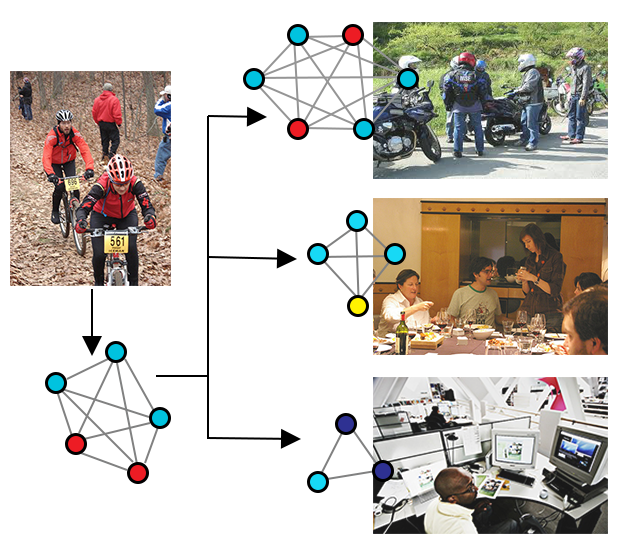
\includegraphics[width=\linewidth]{Co-Loc-Diagram}
  \caption{A semantic entity co-location graph is first built from the query image (on left). It is then compared for similarity with the graph abstractions of other images (on right). The images on right are arranged based on their relative similarity score, top one being the most similar. For pictorial depiction, colors of the nodes indicate the class an entity belongs to. Here, blue: person, red:bike, yellow:table, purple:TV/computer   }
  \label{fig:C0-Loc-Diagram}
\end{figure}

\\In this paper, we harness this input from machine learning models and build a semantic entity relation graph on top of it to derive a broader understanding of the entire scene. We propose real purpose applications that can  utilise this information for various tasks, under a common and unified framework. Our primary contributions involve:
    \begin{enumerate}
        \item End to End pipeline; from tagging Entities in the image and videos to developing their co-location graph and it's usage in vairous applications.
        \item Building Entity co-location graphs in an efficiently scalable, Map-reduce compatible procedure.
        \item Graphical visualisation of entity co-location pattern.
        \item Analysing video stream for user provided emtity's semantic pattern
        \item Semantic content based image retrieval system using the extracted entity relations.
    \end{enumerate}

The paper is broadly divided into 5 sections. Next section revisits the related work done in this domain and points out their differences from our methodoligy. Section 3 describes the proposed methods. Section 4, 5 present the results and the discussion on it respectively. Section 6 shows the path for further enhancement in future.


\section{Background}

Understanding the image context has been a long standing research objctive. Early works on Scene modeling \cite{scene-modeling} used the procedure which was based on a very low dimensional representation of the scene, that they termed as the "Spatial Envelope". They proposed a set of perceptual dimensions (naturalness, openness, roughness, expansion, ruggedness) caculated using spectral and coarsely localized information, that helped in describing the pre-dominant spatial structure of a scene. On other hand, other works aimed at extending GIST \cite{gist}, SIFT{\cite{sift} and other shallow descriptors to derive an overall sense of the image scene.  Beyond Bag of Features \cite{beyondBOW} partitioned the image into increasingly fine sub-regions and computed histograms of local features within each sub-region. The resultant "spatial pyramid" was used for final scene classification. Further work on describing objects by their properties  \cite{image-description} utilised HOG \cite{HOG} features to classify based on understanding fine attributes like furry, spotty, quadrupedal etc of the object. Current models \cite{cnn} \cite{fcnn} \cite{scene-rcnn} \cite{scene-rnn} \cite{scene-lstm}  make heavy use of convolutional and recurrent neural networks for parsing and understanding the overall scene.

Entity information in a single image can be used in videos for understanding each frame and identifying other entities in the upcoming frame with more accuracy probablistically. Such information is critical for surveillance purpose and video classification tasks. Early works \cite{semantic-video-surveillance} utilised  moving object information to track and cluster the trajectories throughout the video.  Mid level features with hierarchical behaviour model was further used for event detection and recognition in semantically annotating video \cite{semantic-video-annotation}. Recent works \cite{video-cnn} \cite{video-to-text} use deep neural nets for classifying videos as well as genrating descriptions out of it based on the entities identified during th run time. Our work primary deals with visualising the entity location pattern from frame to frame basis rather than an overall one for the entire video.

Developing semantic graph layer on top of images have been successfully utilised by researchers in past for utilising the extracted attributs from the scene and developing applications on top of it. BabyTalk \cite{babytalk} constructed a CRF graph on top of entities detected in an image and trained their N-gram language model to generate description based on that. On the other hand, Fang and Lorenzo \cite{semantic-image-distance} created a semantic graph from labeled dataset where the nodes are the labeled images and the edges connect pictures with related labels. This graph was then used for content based image retreival by embedding the query image in the graph and retreiving other images nodes in proximity. Some methods  \cite{semantic-image-tag}  \cite{semantic-graph} aimed at combining both the low/mid level features of the images with that of the text based tags provided by the users. A semantic graph was made by the joint function of above features and was looked up for similar images when provided with a query image. Since it's hard to pre-determine all possible set of input query and it's corresponding classes, weak image ranking schemes \cite{weak-image-rank} have also been researched upon. Such weak features are a collection of mid-level representations, which cancomprise of automatic classifier scores derived through unsupervised learning. Weak attributes are applied to such image retrieval problems by modeling dependency of attributes in query image on weak attributes under the framework of structural learning. Image ranking has been further studied \cite{multi-attribute-image-rank} at even finer feature details. The work goes as far as utilising sub attributes of single object, such as race, color, hair-style etc. for human faces. Owing to lack of such fine details for all the possible entities, the usage of it still remains limited.

\\The work that most closely aligns with our work was shown by Attrbute-Graph \cite{attribute-graph}. Similar to our model, the work builds upon state of the art object detectors to extract the entities present. To build a semantic graph, the authors delve in embedding details ranging from important objects, appearances, spatial layout and background context. This is further augmented with a global node to classify the entire scene. Often for real time problems, computation resources are limited and performing computation on features which don't contribute majorly towards output should be minimized. We see our work as between the models that provide classification for entire image and the ones that go into complete details of every sub attribute of entities. To make complete use of distributed systems and reduce computation time  \cite{map-reduce-image}, our proposed method is designed such that it can be scaled under the map-reduce framework and scale gracefully.

\section{Methods}
Our proposed system can be broadly divided in 5 parts: 
    \begin{enumerate}
            \item The Entity tagger
            \item Extracting co-location graph
            \item Scoring function
            \item Building the cached database for CBIR or Pattern based video stream analysis, depending on the use case. 
            \item Visualing the results in an intuitive and user-friendly way
    \end{enumerate}

    
    \subsection{The Entity Tagger}
        This section is completely independent of the pipeline and can be replaced with any state of the art object detection technique to keep the final results of the application updated. For the current system we have used the YOLO detector because of it's speed and unified detection and localisation abilities. \\ \\
        The network design of it's framework is inspired by the GoogLeNet model for image classification. It is first pre-trained on the ImageNet\cite{imagenet} and then the entire model with additional four convolutional layers on top is fine tuned by training it on the PASCAL VOC 2012 \cite{pascal-voc-2012} dataset which consists of 20 entity categories. It divides the entire image in S*S grid and predicts B bounding boxes for each section. Each bounding box contains 5 items: x,y, width, height and IoU conficence. The centre co-ordinates(x,y) are normalised in the range of 0-1 relative to the corresponding section, whereas the width and height are normalised in the range of 0-1 relative to the width and height of the input image. It also predicts the class probablities for C classes in each section. This enables it to predict the classes of the objects and their respective locations in the image simultaneously. The figure
        \ref{fig:YOLO} shows the entire architecture of the Neural Network used by YOLO.
        The final tensor output of the network is of size: 
        \begin{equation}
            S * S * ( B * 5 + C )
        \end{equation}
        For evaluating YOLO on PASCAL VOC, the values used were S = 7, B = 2. PASCAL VOC has 20 labelled classes so C = 20. Final prediction is a 7x7x30 tensor. To keep the model stable during training phase of reducing the sum-squared error, variables 
        $ \lambda _{coord} = 5$ and $ \lambda_{noobj} = 0.5 $
        are introduced to avoid low confidence boxes from overpowering the gradient. Since slight error in large boxes are less critical than slight error in smaller ones, squared root of width and height are predicted to partially overcome this problem. The network is trained to optimize the following multi-part loss function: \\
        \begin{equation}
        \lambda_{coord} \sum_{i=0}^{S^2} \sum_{j=0}^{B} \mathbb{1}_{ij}^{obj}(x_{i} - \hat x_{i})^{2} + (y_{i} - \hat y_{i})^{2} \\
        
        +  \lambda_{coord} \sum_{i=0}^{S^2} \sum_{j=0}^{B} \mathbb{1}_{ij}^{obj} (\sqrt{ w_{i}} - \sqrt{\hat w_{i}})^{2} + (\sqrt{h_{i}} - \sqrt{\hat y_{i}})^{2} \\
        
        +  \sum_{i=0}^{S^2} \sum_{j=0}^{B} \mathbb{1}_{ij}^{obj}(C_{i} - \hat C_{i})^{2} \\
        
        +  \lambda_{noobj} \sum_{i=0}^{S^2} \sum_{j=0}^{B} \mathbb{1}_{ij}^{obj}(C_{i} - \hat C_{i})^{2} \\
        
        +  \sum_{i=0}^{S^2} \mathbb{1}_{i}^{obj} \sum_{c \in classes} (p_{i}(c) - \hat p_{i}(c))^{2}
        \end{equation}
        
       where $ \mathbb{1}^{obj}_{i} $ denotes if object appears in cell i and $ \mathbb{1}_{ij} $ de-
        notes that the jth bounding box predictor in cell $i$ is “responsible” for that prediction. Thus 98 spatially diverse boxes are proposed anf filtered based on the confidence threshold. Further, non maximal supression is applied to remove the redundant boxes and leverage the accuracy. Final result is an array of objects containing the predicted entities and their respective locations in the image.
        


\begin{figure}
  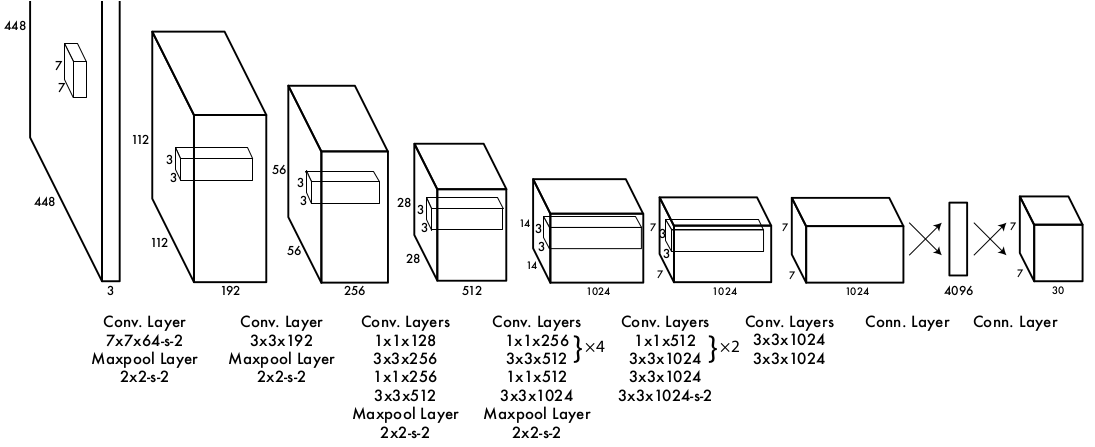
\includegraphics[width=\linewidth]{YOLO}
  \caption{YOLO \cite{yolo} neural network architecture.}
  \label{fig:YOLO}
\end{figure}

    \subsection{Extracting co-location graph}
        
    All the entities in the image are represented as individual nodes on the graph with a unique identity tag. They all share an weighted edge with each other such that value of the edge represent the perceived distance between the entities. It needs to be noted here that since 2 dimensional images themselves have no information about depth, it is practically not possible to accurately identify the actual distance. We use a crude approximation that works well for general images but is susceptible to wrong measurement in case of images that have optical illusion. We pre-assign a relative size value to each entity which our classifier can detect, assuming they all are at the same depth, then we use the following model to estimate the distnce: <Insert equation>. The graphs can then be exported to common formats to maintian cross-compatibility and to have a richer visualisation through other popular frameworks such as Gephi \cite{gephi}.
    
    \subsection{Scoring Function}
    We find the similarity in the abstarcted graphs using the following two part scoring function:     
        \begin{equation}
        FinalScore = \beta * CountDiff + (1 - \beta)*LocDiff
        \label{score}
        \end{equation}
        Here, $\beta \in (0,1)$. The final score is weighted sum of both the scores descrbed below. The parameters $\beta$ help in contolling how much of Entity count similarity should be valued relative to the location differnece score.
        \subsubsection{Entity count score}
        With the objective being to find images which have both the categories and their respective count  as similar to the input image, we first create a vector having $C$ bins. Where $C$ is the number of classes for entities that our classifier can detect. Each bin contains the number of entities belonging to that class in the given image. We then use the weighted sum of squares error to get the similarity score. The weights are dynamically chosen such that for count difference of entity classes present in the image are given priority over count differnece for other entities which are absent in the input image.\\
            \begin{equation}
            CountDiff =  \sum_{i=0}^{C-1} W_{i}*(Inp_{i} - Data_{i})^{2}
            \end{equation}
            \[
              W_{i} = 
              \begin{cases} 
               \alpha & \text{if } Inp_{i} > 0 \\
               1       & \text{if } Inp_{i} = 0
              \end{cases}
            \]
            $\alpha $ governs how much should inter-class entity difference shuld effect the score. In our experiments we found it useful to keep it close to 10. Therefore the lesser the $CountDiff$, the greater is similarity.
        
    \subsubsection{Co-location score}
    To encorporate the notion of co-Location between the objects and score the images that demonstrate similar co-Location pattern as per the query image, we compare the the edge weights of the entity clique using the following function:
        \begin{equation}
        LocDiff = \sum \log (1 + |InpEdge - DataEdge|)
        \end{equation}
    Since the weights are only crude estimations of the visual distance between the entities, we use the logarithm function to reduce the effect of difference on the score.
    
    \subsection{Building cached database for CBIR}
    To facilitate efficient scalability, we use a model similar to the inverse word mapping \cite{map-reduce-inverted-index} \cite{map-reduce-image} that can exploit the power of map reduce on distributed systems. In our model, we use the entity as the key and the values are the corresponding images in which they occur. After a final reduction we get a table which can be quickly looked up to retrieve the images containing the required entity(ies). The set of all the mathced images are then scored according to above mentioned function \ref{score}. 

    \subsection{Video stream analysis}
    This can be used for active search of co-occurence pattern from any video stream. Since it works directly on all the incoming image frames from the video stream, no database is directly involved. Given a query of co-locaton pattern or an image, the system notifies the user automaticaly when similar pattern is encountered in the video. It has vast potential to be deployed in surveillance cameras to automatically raise an alert if a crowd gathers unexpectedly or any peculiar pattern occurs which in anomalous to the area under surveillance. The same scoring function can be used for this task as well.

\section{Results}


\section{Discussions}
    \begin{itemize}
        \item Since the images used in the pipeline are only 2 dimensional and have no depth information, it is not possible to compute the actual distance between any two entities accurately.
        \item YOLO has architecture limitations of locating all the entities which are very close to each other, example: a flock of birds. Other classifiers like SSD\cite{ssd}, Overfeat\cite{overfeat}, Faster R-CNN \cite{faster-rcnn} etc. can  used to overcome this issue.
    \end{itemize}

\section{Future Works}
There is vast scope of expanding the representational power of these semantic graphs. More attributes about the entites like the color of clothes(if it is a person), position in previous frame, time and location co-ordinates, etc can enhance the co-occurence capabilities. These richer features can also help in probablistically identifying same entity across various frames/images. In our current work, only 20 entity classes were used for classification, we can extend it to incorporate more number of classes to obtain a dense represntation of underlying images.
% An example of a floating figure using the graphicx package.
% Note that \label must occur AFTER (or within) \caption.
% For figures, \caption should occur after the \includegraphics.
% Note that IEEEtran v1.7 and later has special internal code that
% is designed to preserve the operation of \label within \caption
% even when the captionsoff option is in effect. However, because
% of issues like this, it may be the safest practice to put all your
% \label just after \caption rather than within \caption{}.
%
% Reminder: the "draftcls" or "draftclsnofoot", not "draft", class
% option should be used if it is desired that the figures are to be
% displayed while in draft mode.
%
%\begin{figure}[!t]
%\centering
%\includegraphics[width=2.5in]{myfigure}
% where an .eps filename suffix will be assumed under latex, 
% and a .pdf suffix will be assumed for pdflatex; or what has been declared
% via \DeclareGraphicsExtensions.
%\caption{Simulation Results}
%\label{fig_sim}
%\end{figure}

% Note that IEEE typically puts floats only at the top, even when this
% results in a large percentage of a column being occupied by floats.


% An example of a double column floating figure using two subfigures.
% (The subfig.sty package must be loaded for this to work.)
% The subfigure \label commands are set within each subfloat command, the
% \label for the overall figure must come after \caption.
% \hfil must be used as a separator to get equal spacing.
% The subfigure.sty package works much the same way, except \subfigure is
% used instead of \subfloat.
%
%\begin{figure*}[!t]
%\centerline{\subfloat[Case I]\includegraphics[width=2.5in]{subfigcase1}%
%\label{fig_first_case}}
%\hfil
%\subfloat[Case II]{\includegraphics[width=2.5in]{subfigcase2}%
%\label{fig_second_case}}}
%\caption{Simulation results}
%\label{fig_sim}
%\end{figure*}
%
% Note that often IEEE papers with subfigures do not employ subfigure
% captions (using the optional argument to \subfloat), but instead will
% reference/describe all of them (a), (b), etc., within the main caption.


% An example of a floating table. Note that, for IEEE style tables, the 
% \caption command should come BEFORE the table. Table text will default to
% \footnotesize as IEEE normally uses this smaller font for tables.
% The \label must come after \caption as always.
%
%\begin{table}[!t]
%% increase table row spacing, adjust to taste
%\renewcommand{\arraystretch}{1.3}
% if using array.sty, it might be a good idea to tweak the value of
% \extrarowheight as needed to properly center the text within the cells
%\caption{An Example of a Table}
%\label{table_example}
%\centering
%% Some packages, such as MDW tools, offer better commands for making tables
%% than the plain LaTeX2e tabular which is used here.
%\begin{tabular}{|c||c|}
%\hline
%One & Two\\
%\hline
%Three & Four\\
%\hline
%\end{tabular}
%\end{table}


% Note that IEEE does not put floats in the very first column - or typically
% anywhere on the first page for that matter. Also, in-text middle ("here")
% positioning is not used. Most IEEE journals/conferences use top floats
% exclusively. Note that, LaTeX2e, unlike IEEE journals/conferences, places
% footnotes above bottom floats. This can be corrected via the \fnbelowfloat
% command of the stfloats package.



\section{Conclusion}
We presented a novel methodology to extract the semantic based entity graph from the image and perform various analysis tasks on it. It is a step forward in harnessing the advancements in the deep learning community and enhancing real world applications. Our method demonstrate more robustness as compared to ones based on only visual similarity and present the users with more sophisticated tools for their tasks.The source code is built using Tensorflow \cite{tensorflow} and OpenCV\cite{opencv}and is openly available to promote future enhancements and collaborations.


% conference papers do not normally have an appendix


% use section* for acknowledgement
\section*{Acknowledgment}


This paper was written when the first author was visiting the CNRS Joint Research Unit of University of Technology of Troyes as a short-term intern on the project CyberSec (Research's Platform in Cyber-security).





% trigger a \newpage just before the given reference
% number - used to balance the columns on the last page
% adjust value as needed - may need to be readjusted if
% the document is modified later
%\IEEEtriggeratref{8}
% The "triggered" command can be changed if desired:
%\IEEEtriggercmd{\enlargethispage{-5in}}

% references section

% can use a bibliography generated by BibTeX as a .bbl file
% BibTeX documentation can be easily obtained at:
% http://www.ctan.org/tex-archive/biblio/bibtex/contrib/doc/
% The IEEEtran BibTeX style support page is at:
% http://www.michaelshell.org/tex/ieeetran/bibtex/
\nocite{*}
\def\BibTeX{BibTeX}
\bibliographystyle{IEEEtran}
% argument is your BibTeX string definitions and bibliography database(s)
\bibliography{IEEEabrv,./IEEEexample}
%
% <OR> manually copy in the resultant .bbl file
% set second argument of \begin to the number of references
% (used to reserve space for the reference number labels box)
%\begin{thebibliography}{1}

%\bibitem{IEEEhowto:kopka}
%H.~Kopka and P.~W. Daly, \emph{A Guide to \LaTeX}, 3rd~ed.\hskip 1em plus
%  0.5em minus 0.4em\relax Harlow, England: Addison-Wesley, 1999.

%\end{thebibliography}




% that's all folks
\end{document}


